\documentclass[a4paper, papersize, dvipdfmx, 12pt, fleqn, bold, ideographic]{jsarticle}
\usepackage{exam_p}
\begin{document}
\section{20}
\fstyle{KRoman}

\subsection{}
以下の\f{1}から\f{10}について適当な式,または文章を入れなさい。
\f{6}については根拠を添えて理由を記述せよ。\f{10}は具体的な数値を含んだ式を書くこと。
\ff{ }は既出の空欄を示す。

\bigskip % 入れた方が見栄えがいい

図に文字を入れる時は,文字のサイズは変更しない。変わりに,\textbf{図のサイズを変更する}。
この時に,図の線の太さが変わり得るので,全選択した後に1ptに設定する。

図を入れる時は\verb|scale=1|で入れるのが最も良い(指定しなくてもok)。

\begin{figure}[ht]
  \centering
  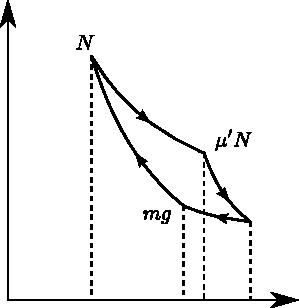
\includegraphics[scale=1]{fig1A_1.pdf}
  \caption{}
  \label{1A.1}
\end{figure}

図を参照する場合は,\verb|\ref{1A.1}|みたいにする:図\ref{1A.1}から...

数式の番号はデフォルトは丸数字になる:
\begin{align}
  F=ma\label{eq1A.1}
\end{align}

参照する場合は\verb|\eqref|を使う:\eqref{eq1A.1}から...

詳しい話はwikiの方も参照してください。面倒な作業はだいたい自動化されてます。
不明なことがあれば開発者に聞きましょう。(自動化されている物をわざわざ手動でやることほど無駄なことは無い)

\newpage

\emptypage

\subsection{}
以下の\f{11}から\f{15}について適当な式,または文章を入れなさい。
\ff{ }は既出の空欄を示す。

[B]を作る人は,自分の番号が何番からスタートするか把握しときましょう。

\end{document}
